\chapter{Captura de requisitos}
%\newpage
%Que tiene que cumplir el trabajo que se va a desarrollar, 
%que necesidades tiene que satisfacer, quienes van a ser sus usuarios, etc.
%
%En un trabajo de desarrollo de software tradicional se 
%documentará mediante el Modelo de casos de uso y la jerarquía 
%de actores, acompañando cada caso de uso y cada actor de una pequeña definición.

\section{Diagrama de casos de uso}
En el diagrama de casos de uso, se puede ver que acciones puede realizar el usuario en cualquier momento, y cuales
est\'an supeditadas a ciertas condiciones. N\'otese que las condiciones de los ``extend" \ son los comentarios a\~nadidos
a los subcasos de uso.

\begin{figure}[h]
\centering
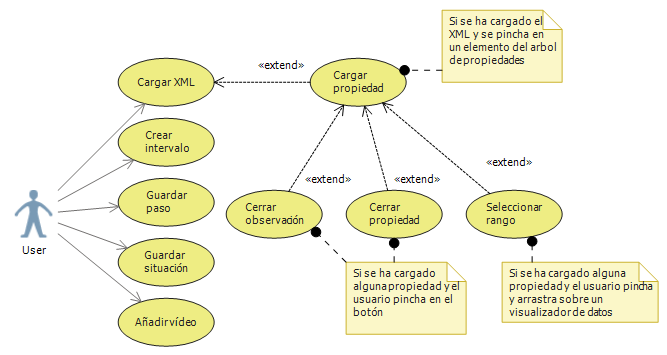
\includegraphics[width=1.0\linewidth]{./Figures/useCaseDiagram.png}
\caption[Diagrama de casos de uso]{Diagrama de casos de uso}
\label{fig:useCaseDiagram}
\end{figure}

\subsection{Casos de uso extendidos}
En esta secci\'on se proceder\'a a explicar brevemente cada caso de uso. %, dar una descripci\'on
%de que se hace, que actores toman parte, precondiciones, requisitos no funcionales, el flujo de
%eventos, as\'i como sus poscondiciones e interfaz gr\'afica asociada.

\subsubsection{Cargar XML}

\begin{table}[H]
	\begin{center}
		\rowcolors{2}{lightgray}{} %\rowcolors{<starting row index>}{<odd row color>}{<even row color>}
		\begin{tabular}{|l*{1}{p{10cm}}|}
			
			\multicolumn{2}{c}{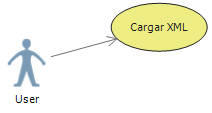
\includegraphics[width=0.4\linewidth]{./Figures/CargarXML.png}} \\
			\hline
		    Nombre                     & Cargar XML \\
		    Descripci\'on              & Carga un XML que contiene las propiedades
		    							 y las observaciones en el sistema. \'Unicamente
		    							 se cargan si el archivo valida contra el XSD.  \\ 
		    Actores                    & User  \\
		    Precondiciones             & Ninguna  \\
		    Requisitos no funcionales  & Ninguno  \\
		    Flujo de eventos           & \begin{enumerate}
		    								\item El usuario pincha en File -> Load XML.
		    								\item Se abre una ventana de selecci\'on de archivos.
		    								\item \textbf{Si el usuario quiere cargar un fichero}
		    								\begin{enumerate}
		    									\item Lo busca en el sistema de archivos
		    									\item Lo selecciona y pincha en Abrir.
		    									
		    									\item \textbf{Si es un documento v\'alido}
		    									\begin{enumerate}
		    										\item Las observaciones y sus propiedades 
		    											  aparecen en el \'arbol lateral.
		    									\end{enumerate}
		    									\item \textbf{Si no}
		    									\begin{enumerate}
		    										\item Se muestra un error.
		    									\end{enumerate}
		    								\end{enumerate}
		    								\item \textbf{Si no desea cargarlo}
		    								\begin{enumerate}
		    									\item Pincha en cancelar.
		    								\end{enumerate}
		    							 \end{enumerate} \\
		    Poscondiciones			   & El \'arbol contendr\'a las observaciones y 
		    							 propiedades si era un documento v\'alido, mostrar\'a
		    							 un error si era un documento inv\'alido, o no 
		    							 suceder\'a nada si el usuario ha decidido no cargar
		    							 el fichero.  \\
		    Interfaz gr\'afica		   & Figuras \ref{fig:Alcance}, \ref{fig:Scrum},
		    							 \ref{fig:Alcance}, \ref{fig:Scrum} y \ref{fig:Alcance}\\
		    \hline
		\end{tabular}
	\caption[Cargar XML]{Cargar XML}
	\label{Cargar XML}
	\end{center}
\end{table}

\subsubsection{A\~nadir v\'ideo}

\begin{table}[H]
	\begin{center}
		\rowcolors{2}{lightgray}{} %\rowcolors{<starting row index>}{<odd row color>}{<even row color>}
		\begin{tabular}{|l*{1}{p{10cm}}|}
			
			\multicolumn{2}{c}{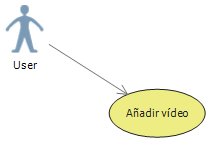
\includegraphics[width=0.4\linewidth]{./Figures/AnadirVideo.png}} \\
			\hline
		    Nombre                     & A\~nadir v\'ideo \\
		    Descripci\'on              & Abre un v\'ideo y lo a\~nade al contenedor
		    							 de v\'ideos si ya hab\'ia v\'ideos previamente
		    							 cargados. Si no, a\~nade tambi\'en un contenedor
		    							 de v\'ideos.  \\ 
		    Actores                    & User  \\
		    Precondiciones             & Ninguna  \\
		    Requisitos no funcionales  & Ninguno  \\
		    Flujo de eventos           & \begin{enumerate}
		    								\item El usuario pincha en Add Video.
		    								\item Se abre una ventana de selecci\'on de archivos.
		    								\item \textbf{Si el usuario quiere cargar un v\'ideo}
		    								\begin{enumerate}
		    									\item Lo busca en el sistema de archivos
		    									\item Lo selecciona y pincha en Abrir.
		    									
		    									\item \textbf{Si el contenedor de v\'ideos estaba
		    												  cargado}
		    									\begin{enumerate}
		    										\item Se a\~nade el v\'ideo al contenedor
		    											  existente.
		    									\end{enumerate}
		    									\item \textbf{Si no}
		    									\begin{enumerate}
		    										\item Se crea y a\~nade un contenedor de v\'ideos y se le a\~nade el nuevo v\'ideo.
		    									\end{enumerate}
		    								\end{enumerate}
		    								\item \textbf{Si no desea cargarlo}
		    								\begin{enumerate}
		    									\item Pincha en cancelar.
		    								\end{enumerate}
		    							 \end{enumerate} \\
		    Poscondiciones			   & El contenedor con el nuevo v\'ideo a\~nadido  \\
		    Interfaz gr\'afica		   & Figuras \ref{fig:Alcance}, \ref{fig:Scrum},
		    							 \ref{fig:Alcance}, \ref{fig:Scrum} y \ref{fig:Alcance}\\
		    \hline
		\end{tabular}
	\caption[A\~nadir v\'ideo]{A\~nadir v\'ideo}
	\label{Anadir video}
	\end{center}
\end{table}
\pagebreak

\subsubsection{Cargar propiedad}

\begin{table}[H]
	\begin{center}
		\rowcolors{2}{lightgray}{} %\rowcolors{<starting row index>}{<odd row color>}{<even row color>}
		\begin{tabular}{|l*{1}{p{10cm}}|}
			
			\multicolumn{2}{c}{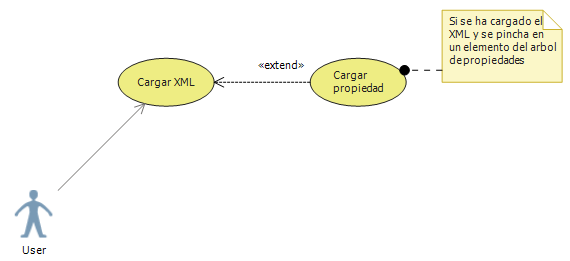
\includegraphics[width=1.0\linewidth]{./Figures/CargarPropiedad.png}} \\
			\hline
		    Nombre                     & Cargar propiedad \\
		    Descripci\'on              & Carga una propiedad en el contenedor de gr\'aficos
		    							 correspondiente a la observaci\'on a la que pertenece.
		    							 Tambi\'en puede a\~nadir propiedades en grupo, haciendo
		    							 doble click sobre el nombre de la observaci\'on. Si
		    							 el contenedor no est\'a creado, lo crea.  \\ 
		    Actores                    & User  \\
		    Precondiciones             & Ninguna  \\
		    Requisitos no funcionales  & Ninguno  \\
		    Flujo de eventos           & \begin{enumerate}
		    								\item El usuario hace doble click en alg\'un elemento
		    									  del \'arbol de observaciones y propiedades.
		    								\item \textbf{Si el elemento es una observaci\'on}
		    								\begin{enumerate}
		    									\item Carga el contenedor si no estaba creado
		    									\item A\~nade todos sus hijos no cargados al
		    										  contenedor.
		    								\end{enumerate}
		    								\item \textbf{Si el elemento es una propiedad}
		    								\begin{enumerate}
			    								\item Crea el contenedor de la observaci\'on
			    									  a la que pertenece la propiedad seleccionada
			    									  si no estaba cargado.
			    								\item A\~nade la propiedad si no estaba cargada
			    									  previamente.
			    									  
		    								\end{enumerate}
		    							 \end{enumerate} \\
		    Poscondiciones			   & El contenedor de la observaci\'on y todas las 
		    							 propiedades de la observaci\'on o la propiedad
		    							 seleccionada dependiendo de donde se haya hecho 
		    							 doble click y sincronizada con el rango existente, si es que lo hay. \\
		    Interfaz gr\'afica		   & Figuras \ref{fig:Alcance}, \ref{fig:Scrum},
		    							 \ref{fig:Alcance}, \ref{fig:Scrum} y \ref{fig:Alcance}\\
		    \hline
		\end{tabular}
	\caption[Cargar propiedad]{Cargar propiedad}
	\label{Cargar propiedad}
	\end{center}
\end{table}
\pagebreak

\subsubsection{Seleccionar rango}

\begin{table}[H]
	\begin{center}
		\rowcolors{2}{lightgray}{} %\rowcolors{<starting row index>}{<odd row color>}{<even row color>}
		\begin{tabular}{|l*{1}{p{10cm}}|}
			
			\multicolumn{2}{c}{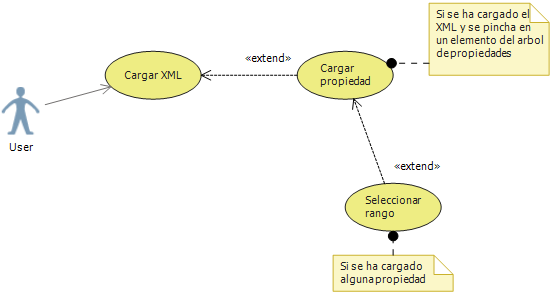
\includegraphics[width=1.0\linewidth]{./Figures/SeleccionarRango.png}} \\
			\hline
		    Nombre                     & Seleccionar rango \\
		    Descripci\'on              & Al pinchar y mover el rat\'on sobre un visualizador de datos,
		    							 se seleccionar\'a un rango en todos los visualizadores de datos
		    							 cargados en el sistema. \\ 
		    Actores                    & User  \\
		    Precondiciones             & Alguna propiedad tiene que estar cargada  \\
		    Requisitos no funcionales  & Ninguno  \\
		    Flujo de eventos           & \begin{enumerate}
		    								\item El usuario pincha en un visualizador de datos.
		    								\item El usuario arrastra (manteniendo pinchado) el rat\'on.
		    								\begin{enumerate}
		    									\item Cada vez que el rango seleccionado cambia, se notifica al contenedor padre.
		    									\item El contenedor, notifica al repositorio de contenedores, para que todos
		    									se sincronicen con el dato proporciado.
		    									\item Se recorren todos los visualizadores de datos para sincronizarse con el nuevo
		    									valor.
		    								\end{enumerate}
		    								\item El usuario deja de pinchar, y se queda el rango seleccionado
		    							 \end{enumerate} \\
		    Poscondiciones			   & El rango quedar\'a seleccionado en todos los visualizadores de datos
		    							 cargados en el sistema.  \\
		    Interfaz gr\'afica		   & Figuras \ref{fig:Alcance}, \ref{fig:Scrum},
		    							 \ref{fig:Alcance}, \ref{fig:Scrum} y \ref{fig:Alcance}\\
		    \hline
		\end{tabular}
	\caption[Seleccionar rango]{Seleccionar rango}
	\label{SeleccionarRango}
	\end{center}
\end{table}
\pagebreak

\subsubsection{Cerrar observaci\'on}
\begin{table}[H]
	\begin{center}
		\rowcolors{2}{lightgray}{} %\rowcolors{<starting row index>}{<odd row color>}{<even row color>}
		\begin{tabular}{|l*{1}{p{10cm}}|}
			
			\multicolumn{2}{c}{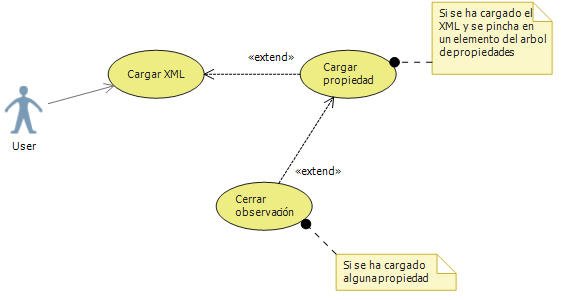
\includegraphics[width=1.0\linewidth]{./Figures/CerrarObservacion.png}} \\
			\hline
		    Nombre                     & Cerrar observaci\'on \\
		    Descripci\'on              & Elimina, tanto de manera visual, como de memoria, la observaci\'on
		    							 seleccionada y todos sus visualizadores de datos (propiedades) asociadas  \\ 
		    Actores                    & User  \\
		    Precondiciones             & La observaci\'on ten\'ia que estar cargada. \\
		    Requisitos no funcionales  & Ninguno  \\
		    Flujo de eventos           & \begin{enumerate}
		    								\item El usuario pincha sobre la ``X" \ en la esquina
		    									  superior derecha de la observaci\'on.
		    								\item Se borra del repositorio, liberando sus recursos, y con ello,
		    									  sus propiedades.
		    								\item Finalmente se borra de la pantalla.
		    							 \end{enumerate} \\
		    Poscondiciones			   & El espacio de trabajo contendr\'a todas las observaciones
		    							 y propiedades menos la que se ha cerrado.  \\
		    Interfaz gr\'afica		   & Figuras \ref{fig:Alcance}, \ref{fig:Scrum},
		    							 \ref{fig:Alcance}, \ref{fig:Scrum} y \ref{fig:Alcance}\\
		    \hline
		\end{tabular}
	\caption[Cerrar observaci\'on]{Cerrar observaci\'on}
	\label{Cerrar observacion}
	\end{center}
\end{table}
\pagebreak

\subsubsection{Cerrar propiedad}

\begin{table}[H]
	\begin{center}
		\rowcolors{2}{lightgray}{} %\rowcolors{<starting row index>}{<odd row color>}{<even row color>}
		\begin{tabular}{|l*{1}{p{10cm}}|}
			
			\multicolumn{2}{c}{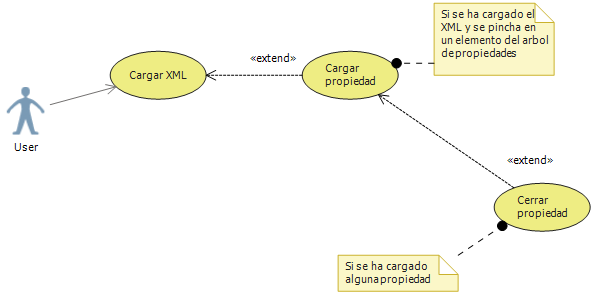
\includegraphics[width=1.0\linewidth]{./Figures/CerrarPropiedad.png}} \\
			\hline
			Nombre                     & Cerrar propiedad \\
			Descripci\'on              & Elimina, tanto de manera visual, como de memoria, la propiedad
									  	 seleccionada.  \\ 
			Actores                    & User.  \\
			Precondiciones             & La propiedad ten\'ia que estar cargada. \\
			Requisitos no funcionales  & Ninguno.  \\
			Flujo de eventos           & \begin{enumerate}
										 	\item El usuario pincha sobre la ``X" \ en la esquina
												  superior derecha de la propiedad.
											\item Se borra del contenedor al que estaba asociada.
											\item Finalmente se borra de la pantalla.
										 \end{enumerate} \\
			Poscondiciones			   & El espacio de trabajo contendr\'a todas las observaciones
										 y propiedades menos la propiedad que se ha cerrado.  \\
			Interfaz gr\'afica		   & Figuras \ref{fig:Alcance}, \ref{fig:Scrum},
			\ref{fig:Alcance}, \ref{fig:Scrum} y \ref{fig:Alcance}\\
			\hline
		\end{tabular}
	\caption[Cerrar propiedad]{Cerrar propiedad}
	\label{Cerrar propiedad}
	\end{center}
\end{table}

\subsubsection{Guardar intervalo}

\begin{table}[H]
	\begin{center}
		\rowcolors{2}{lightgray}{} %\rowcolors{<starting row index>}{<odd row color>}{<even row color>}
		\begin{tabular}{|l*{1}{p{10cm}}|}
			
			\multicolumn{2}{c}{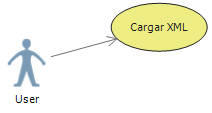
\includegraphics[width=0.4\linewidth]{./Figures/CargarXML.png}} \\
			\hline
		    Nombre                     & Guardar intervalo \\
		    Descripci\'on              & A\~nade el intervalo seleccionado
		    							 a los intervalos a guardar en el xml si
		    							 no se superpone con los que ya est\'an guardados.  \\ 
		    Actores                    & User  \\
		    Precondiciones             & Ninguna  \\
		    Requisitos no funcionales  & Ninguno  \\
		    Flujo de eventos           & \begin{enumerate}
		    								\item El usuario pincha en File -> Load XML.
		    								\item Se abre una ventana de selecci\'on de archivos.
		    								\item \textbf{Si el usuario quiere cargar un fichero}
		    								\begin{enumerate}
		    									\item Lo busca en el sistema de archivos
		    									\item Lo selecciona y pincha en Abrir.
		    									
		    									\item \textbf{Si es un documento v\'alido}
		    									\begin{enumerate}
		    										\item Las observaciones y sus propiedades 
		    											  aparecen en el \'arbol lateral.
		    									\end{enumerate}
		    									\item \textbf{Si no}
		    									\begin{enumerate}
		    										\item Se muestra un error.
		    									\end{enumerate}
		    								\end{enumerate}
		    								\item \textbf{Si no desea cargarlo}
		    								\begin{enumerate}
		    									\item Pincha en cancelar.
		    								\end{enumerate}
		    							 \end{enumerate} \\
		    Poscondiciones			   & El \'arbol contendr\'a las observaciones y 
		    							 propiedades si era un documento v\'alido, mostrar\'a
		    							 un error si era un documento inv\'alido, o no 
		    							 suceder\'a nada si el usuario ha decidido no cargar
		    							 el fichero.  \\
		    Interfaz gr\'afica		   & Figuras \ref{fig:Alcance}, \ref{fig:Scrum},
		    							 \ref{fig:Alcance}, \ref{fig:Scrum} y \ref{fig:Alcance}\\
		    \hline
		\end{tabular}
	\caption[Cargar XML]{Cargar XML}
	\label{Cargar XML}
	\end{center}
\end{table}

\section{Modelo de dominio}
Los datos que se guardan son ciertamente bastante simples, ya que para la tripleta Instante, Observaci\'on y Propiedad,
toma un \'unico valor posible. 

La Figura \ref{fig:ModelodeDominio} representa tanto los datos de entrada del software, tanto los datos
de salida.

\begin{figure}[h]
\centering
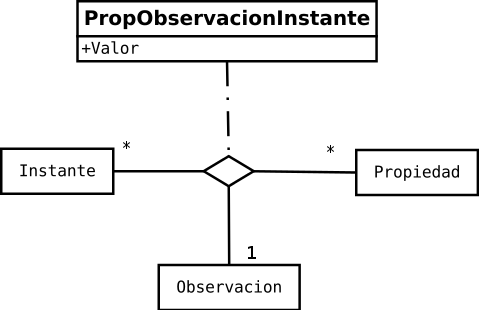
\includegraphics[width=0.7\linewidth]{./Figures/ModelodeDominio}
\caption[Modelo de dominio]{Modelo de dominio}
\label{fig:ModelodeDominio}
\end{figure}
